\chapter{Mathematical models of Bose-Einstein condensates}

In this chapter we provide the theoretical background necessary to understand
the dynamics of ultracold atomic gases.
We start by introducing the most simple form of a Bose-Einstein condensate,
the scalar condensate.
This lays the framework for building to more complex systems.
We then go on to discuss the two-component condensate, where additional
interactions arise between atoms of differing components.
Finally, we construct the framework needed to understand spinor BECs, which is
the main basis of this thesis.

\section{Scalar Bose-Einstein condensates}
\subsection{Mean-field description}
A system of \(N\) particles interacting through binary collisions is described
by an \(N\)-body Schr\"{o}dinger equation, given as
\begin{equation}
    i\hbar \pdv{}{t}\Psi(\vb{r}_1;\ldots;\vb{r}_N, t) =
    \hat{H}_N\Psi(\vb{r}_1;\ldots;\vb{r}_N, t),
\end{equation}
where the \(N\)-body Hamiltonian operator is given by
\begin{equation}
    \hat{H}_N = -\sum_i \frac{\hbar^2}{2m}\nabla_i^2
    + \sum_{i \neq j}V(\vb{r}_i - \vb{r}_j).
\end{equation}
The first sum of the above equation represents the kinetic energy operator,
whilst the second describes the two-body potential operator.
This description, however, becomes unwieldy when trying to model the number of
particles associated with typical BEC experiments.

Instead, we model the system using a mean-field theory, in which we make two
assumptions.
Firstly, the dilute nature of a BEC justifies that any binary interaction
between two particles at positions \(\vb{r}_1, \vb{r}_2\) takes the form of
a contact interaction modelled by the following delta function:
\begin{equation}
    V(\vb{r}_1 - \vb{r}_2) = g\delta(\vb{r}_1 - \vb{r}_2),
\end{equation}
where \(g\) represents an interaction coefficient.
Secondly, we assume that, for sufficiently low temperatures, the system
undergoes Bose-Einstein condensation, and all particles of
the system occupy the same quantum state.
This implies that each particle is described by the same single-particle wave
function and hence the system can be described by a macroscopic wave function
\(\psi(\vb{r}, t)\) for position \(\vb{r}\) and time \(t\).
Additionally, the field \(\psi \) is scalar since each particle shares the same
phase and quantum state.
This approximation is only valid in the limit of zero temperature, where there
are no particles contributing to thermal or quantum fluctuations beyond the
classical field.

\subsection{The Gross-Pitaevskii equation}
The preceding assumptions form the basis of constructing the underlying equation
that governs the dynamics of Bose-Einstein condensate systems: the
Gross-Pitaevskii equation (GPE):
\begin{equation}\label{eq: scalar-GPE}
    i\hbar \pdv{\psi(\vb{r}, t)}{t} = \left(-\frac{\hbar^2}{2m}\nabla^2
    + V(\vb{r}, t) +g|\psi(\vb{r}, t)|^2\right)\psi(\vb{r}, t),
\end{equation}
where \(V(\vb{r}, t)\) is a trapping potential.

The first two terms on the right-hand side describe the energy of a single
particle in an external potential.
The third term accounts for the interactions within the condensate, where
\(g=4\pi \hbar^2a_s/m\) is the interaction strength of the condensate for
s-wave scattering length \(a_s\) and atomic mass \(m\).
For \(g>0\) the interactions are repulsive and for \(g < 0\) attractive.
When \(g=0\) there are no interactions present and the system reduces to the
Schr\"{o}dinger equation.

The wave function of the system is normalised to the number of particles
\begin{equation}
    \int |\psi(\vb{r}, t)|^2 d\vb{r} = N.
\end{equation}
The total mass of the condensate is given as \(M=mN\), where \(N\) is provided
by the above normalisation condition.

The energy of the system is
\begin{equation}
    E = \int d^3\vb{r} \left[\frac{\hbar^2}{2m}|\nabla\psi|^2
        + V|\psi|^2 + \frac{g}{2}|\psi|^4\right]
    = E_\mathrm{kin} + E_\mathrm{pot} + E_\mathrm{int},
\end{equation}
where \(E_\mathrm{kin}, E_\mathrm{pot}\) and \(E_\mathrm{int}\) describes the
kinetic, potential, and interaction energies, respectively.

\section{Two-component Bose-Einstein condensates}
We now generalise part of the theory introduced in the previous section to
describe multi-component condensates.
The time-dependent coupled Gross-Pitaevskii equations each describe a condensate
similar to the standard GPE, but now with an additional non-linear term that
describes the interactions of atoms between condensate components.
The coupled GPEs are given as
\begin{equation}\label{eq: two-component-GPEs}
    \begin{aligned}
        i\hbar \pdv{\psi_1(\vb{r}, t)}{t} & =
        \left[-\frac{\hbar^2}{2m_1}\nabla^2 + V_1(\vb{r}, t)
            + g_1|\psi_1(\vb{r}, t)|^2
        + g_{12}|\psi_2(\vb{r}, t)|^2\right]\psi_1(\vb{r}, t) \\
        i\hbar \pdv{\psi_2(\vb{r}, t)}{t} & =
        \left[-\frac{\hbar^2}{2m_2}\nabla^2 + V_2(\vb{r}, t)
            + g_2|\psi_2(\vb{r}, t)|^2
            + g_{12}|\psi_1(\vb{r}, t)|^2\right]\psi_2(\vb{r}, t),
    \end{aligned}
\end{equation}
where \(\psi_j(\vb{r}, t)\) describes component \(j\) with atomic mass \(m_j\)
for \(j=1, 2\) and \(V(\vb{r}, t)\) is an external trapping potential.
Additionally, the interaction terms are given as
\begin{equation}
    g_j = \frac{4\pi \hbar^2a_j}{2m_j}, \qquad
    g_{12} = g_{21} = \frac{2\pi\hbar^2(m_1+m_2)a_{12}}{m_1m_2},
\end{equation}
which describe the intra-species and inter-species interaction strengths,
respectively.
Similar to the scalar case, the wave function of each component is normalised
to the number of atoms of that component
\begin{equation}
    \int |\psi_j|^2 d^3\vb{r} = N_j.
\end{equation}

The time-independent GPEs are obtained through the substitution
\(\psi_j(\vb{r}, t)=\psi_j(\vb{r})e^{-i\mu_j t/\hbar}\) in
Eq.~\eqref{eq: two-component-GPEs}, yielding
\begin{equation}\label{eq: time-indep-two-component-GPEs}
    \begin{aligned}
        \mu_1\psi_1(\vb{r}) & =
        \left[-\frac{\hbar^2}{2m_1}\nabla^2 + V_1(\vb{r})
            + g_1|\psi_1(\vb{r})|^2
        + g_{12}|\psi_2(\vb{r})|^2\right]\psi_1(\vb{r}) \\
        \mu_2\psi_2(\vb{r}) & =
        \left[-\frac{\hbar^2}{2m_2}\nabla^2 + V_2(\vb{r})
            + g_2|\psi_2(\vb{r})|^2
            + g_{12}|\psi_1(\vb{r})|^2\right]\psi_2(\vb{r}),
    \end{aligned}
\end{equation}
where \(\mu_j\) is the chemical potential of component \(j\).

The total energy of the two-component system is composed of the contributions
from each component as
\begin{equation}
    \begin{aligned}
        E & = \int \left[\frac{\hbar^2}{2m_1}|\nabla\psi_1|^2
        + V_1|\psi_1|^2 + \frac{g_1}{2}|\psi_1|^2 \right] d^3\vb{r}   \\
          & + \int \left[\frac{\hbar^2}{2m_2}|\nabla\psi_2|^2
        + V_2|\psi_2|^2 + \frac{g_2}{2}|\psi_2|^2 \right] d^3\vb{r}   \\
          & + \int \left[g_{12}|\psi_1|^2|\psi_2|^2\right] d^3\vb{r}.
    \end{aligned}
\end{equation}

\subsection{Miscible and immiscible regimes}
Two-component condensates can either be miscible or immiscible, depending on
the interactions present within the system.
Here, we derive the immiscibility criterion for two-component condensates
following the procedure in Ref.~\cite{Ao1998}.

We start by assuming, for simplicity, a square-well trapping potential with
\(V(\vb{r}) = 0\) inside the well and setting \(V\) to be infinitely large
outside.
Assuming a stationary solution and hence neglecting the kinetic energy
terms, Eq.~\eqref{eq: time-indep-two-component-GPEs} reduce to
\begin{equation}
    \begin{aligned}
        \mu_1 & = g_1|\psi_1|^2 + g_{12}|\psi_2|^2, \\
        \mu_2 & = g_2|\psi_2|^2 + g_{12}|\psi_1|^2.
    \end{aligned}
\end{equation}

Inside the trap the densities of each component can be re-written as
\(n_j=N_j/V\), where \(V\) is the volume of the condensate.
The above equations then reduce to \(g_1n_1 + g_{12}n_2 = \mu_1\) and
\(g_2n_2 + g_{12}n_1 = \mu_2\), and the energy becomes
\begin{equation}
    E_\mathrm{misc} = \frac{1}{2}\left[g_1\frac{N_1^2}{V} + g_2\frac{N_2^2}{V}
        + 2g_{12}\frac{N_1N_2}{V}\right].
\end{equation}
Provided \(g_{12}\) is small enough, any variation to this state will increase
the system energy, implying that this state is stable.
When \(g_{12}\) gets large enough, however, it can be shown that there exists
a state with a lower energy.

Let us consider an immiscible regime, where the two condensates do not spatially
overlap.
The volume of condensate \(j\) is given as \(V_j\) and the densities
subsequently become \(n_j=N_j/V_j\).
Eqs.~\eqref{eq: time-indep-two-component-GPEs} become \(g_j n_j = \mu_j\) with
total energy
\begin{equation}\label{eq: immiscible-energy}
    E_\mathrm{immisc} = \frac{1}{2}\left[g_1\frac{N_1^2}{V_1}
        + g_2\frac{N_2^2}{V_2}\right].
\end{equation}
Minimising the above energy with respect to \(V_1\) or \(V_2\) with
\(V=V_1+V_2\) results in the expressions for the volume of each component
\begin{equation}
    V_1 = \frac{1}{1 + \sqrt{g_2/g_1}(N_2/N_1)}V,
\end{equation}
\begin{equation}
    V_2 = \frac{1}{1 + \sqrt{g_1/g_2}(N_1/N_2)}V.
\end{equation}
The corresponding densities then become
\begin{equation}
    \begin{aligned}
        n_1 = \left(1 + \sqrt{\frac{g_2}{g_1}}\frac{N_2}{N_1}\right)
        \frac{N_1}{V},
        n_2 = \left(1 + \sqrt{\frac{g_1}{g_2}}\frac{N_1}{N_2}\right)
        \frac{N_2}{V}.
    \end{aligned}
\end{equation}
Substituting the above densities into the expression for the total energy
in Eq.~\eqref{eq: immiscible-energy} yields
\begin{equation}
    E_\mathrm{immisc} = \frac{1}{2}\left[g_1\frac{N_1^2}{V} + g_2\frac{N_2^2}{V}
        + 2\sqrt{g_1g_2}\frac{N_1N_2}{V}\right].
\end{equation}

The difference between the energies of the miscible and immiscible phases
is
\begin{equation}
    \Delta E = E_\mathrm{misc} - E_\mathrm{immisc} = (g_{12} - \sqrt{g_1g_2})
    \frac{N_1N_2}{V}
\end{equation}
Therefore, the condition \(g_{12} > \sqrt{g_1g_2}\) reveals that for large
enough inter-species interactions the system favours an immiscible phase
over a miscible one.
This criterion only depends on the interactions within the system, and is not
affected by condensate particle numbers or size.
Fig.~\ref{fig: miscible-vs-immiscible} shows the boundary between the two
phases for \(g_1=1\) in a parameter space of \(g_2, g_{12}\).
\begin{figure}
    \centering
    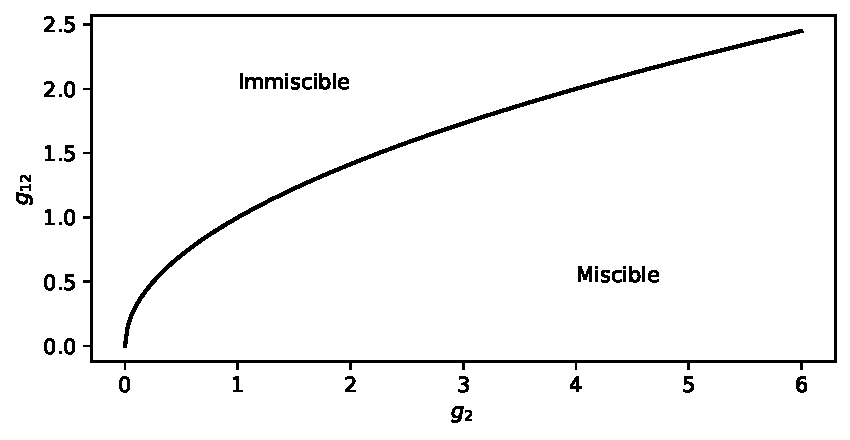
\includegraphics{gfx/ch-theory/miscible_vs_immiscible.pdf}
    \caption[Two-component miscible vs immiscible boundary]
    {\label{fig: miscible-vs-immiscible}Boundary between the miscible
        and immiscible regimes for a two-component condensate with \(g_1=1\).}
\end{figure}


\section{Spinor Bose-Einstein condensates}
Spinor systems comprise particles with total spin \(f\).
This implies there are \(2f + 1\) possible spin states along a given spin
quantisation axis.
Such a state is denoted \(\ket{f, m} \), where
\(m \in \{-f, -f+1, \ldots, 0, \ldots, f - 1, f\} \) denotes the magnetic
sublevel for total spin \( f\).

A general spin-\(f\) state is described by the (\(2f+1\))-component wave
function \(\psi \), defined as \(\ket{\psi} = \sum_m\psi_m\ket{f, m}\).
In the spin-1 case, we have \(\psi = {(\psi_1, \psi_0, \psi_{-1})}^T\), and for
the spin-2 case \(\psi = {(\psi_2, \psi_1, \psi_0, \psi_{-1}, \psi_{-2})}^T\).

Two identical spin-\(f\) bosons (atoms with integer spin) can collide to form a
total spin of \(\EuScript{F} = 0, 2, \ldots, 2f\) depending on the orientation
of the particles, with \(\EuScript{M} \equiv m+m' \in
\{-\EuScript{F}, \ldots, \EuScript{F}\} \).
In the s-wave scattering limit, where the orbital angular momentum is zero,
the total spin of two interacting particles must be even.
Due to the rotational symmetry, the scattering lengths depend only on the total
spin \(\EuScript{F}\), implying there are \(f + 1\) different scattering lengths
\(a_0, a_2, \ldots, a_{2f}\).

In a spinor BEC, the effective contact interaction is generalised to include
contributions from all spin channels as
\begin{equation}\label{eq: spin-f-interaction-potential}
    V_\mathrm{int} = \delta(\vb{r_1} - \vb{r_2})
    \sum_{\EuScript{F}=0}^{2f}g_\EuScript{F}\vb{P}_\EuScript{F},
\end{equation}
where \(g_\EuScript{F}=4\pi\hbar^2a_\EuScript{F}/M\) and
\(\vb{P}_\EuScript{F}\) is the projection operator which projects a pair
of atoms into a total spin \(\EuScript{F}\) state, defined as
\begin{equation}
    \vb{P}_\EuScript{F} = \sum_{m=-\EuScript{F}}^{\EuScript{F}}
    \ket{\EuScript{F}, \EuScript{M}}\bra{\EuScript{F}, \EuScript{M}}.
\end{equation}
For a system of identical bosons, the sum over all projection operators gives
\begin{equation}\label{eq: completeness-relation}
    \sum_{\EuScript{F}=0}^{2f}\vb{P}_\EuScript{F} = 1.
\end{equation}


\subsection{Spin-1 interaction Hamiltonian}\label{subsec: spin-1-int-hamil}
To calculate the spin-dependent mean-field interaction potential, it is common
to relate the projection operators to products of the single-particle spin
operators.
For a spin-1 condensate, the composition law of the angular momentum
gives~\cite{Kawaguchi2012, StamperKurn2013}
\begin{equation}\label{eq: composition-law}
    \vb{F}_1 \cdot \vb{F}_2 = \frac{1}{2}\left[{(\vb{F}_1 + \vb{F}_2)}^2
        - \vb{F}_1^2 - \vb{F}_2^2\right] = \frac{1}{2}\EuScript{F}(\EuScript{F} + 1)
    -f(f+1),
\end{equation}
where \(\vb{F}_i\) is the spin operator for atom \(i\).
From here we can construct the relation \(\vb{F}_1 \cdot \vb{F}_2 =
\sum_{\EuScript{F} = 0}^{2f}\lambda_\EuScript{F}\vb{P}_\EuScript{F}\), where
\(\lambda_\EuScript{F} = \frac{1}{2}\EuScript{F}(\EuScript{F} + 1)
-f(f+1)\).
In an \(f=1\) spinor condensate, only \(\EuScript{F} = 0\) or \(2\) channels
are allowed.
Therefore, we have
\begin{equation}\label{eq: spin-1-spin-relation}
    \vb{F}_1 \cdot \vb{F}_2 = \sum_{\EuScript{F} = 0}^{2f}
    \lambda_\EuScript{F}\vb{P}_\EuScript{F} = \vb{P}_2 - 2\vb{P}_0,
\end{equation}
and
\begin{equation}\label{eq: spin-1-completeness-relation}
    \sum_{\EuScript{F} = 0}^{2f} = 1 = \vb{P}_0 + \vb{P}_2.
\end{equation}
Using both Eq.~\eqref{eq: spin-1-spin-relation} and
Eq.~\eqref{eq: spin-1-completeness-relation}, one can re-write
Eq.~\eqref{eq: spin-f-interaction-potential} as
\begin{equation}
    V_\mathrm{int} = \delta(\vb{r}_1 - \vb{r}_2)
    (c_0 + c_1 \vb{F}_1 \cdot \vb{F}_2),
\end{equation}
where \(c_0 = (g_0+2g_2)/3\) and \(c_1=(g_2-g_0) / 3\).
Finally, the spin-1 interacting Hamiltonian is then given as
\begin{equation}\label{eq: spin-1-interacting-Hamiltonian}
    H_\mathrm{int} = \frac{1}{2}\int d\vb{r} (c_0n^2 + c_1|\vb{F}|^2).
\end{equation}

Here \(c_0\) is interpreted as the spin-independent interaction strength.
It becomes apparent from Eq.~\ref{eq: spin-1-interacting-Hamiltonian} that
\(c_0 > 0\) (repulsive interactions) is required for stability.
In the \(c_0 < 0\) limit (i.e., attractive interactions), the condensate would
favour becoming infinitely dense, and in the process would destroy itself.
Therefore, throughout this thesis we always consider \(c_0 > 0\).

The \(c_1\) term describes is the spin-dependent interaction strength.
Since \(c_0\) is constrained to be positive, \(c_1\) can take positive or
negative values.
When \(c_1 > 0\), the system energetically favours minimising the condensate
spin \(\vb{F}\), which are typically referred to as antiferromagnetic or polar
interactions.
Conversely, for \(c_1 < 0\) the system favours maximising the spin vector,
which are referred to as ferromagnetic interactions.

Finally, we note that since \(c_1\) is the difference of two s-wave scattering
lengths which are comparable in magnitude experimentally, the spin-dependent
interaction strength is usually much smaller than the spin-independent strength.

\subsection{Spin-2 interaction Hamiltonian}
For an \(f=2\) spinor condensate, we now have \(\EuScript{F}=0,2,4\) spin
channels.
For a spin-2 condensate, Eq.~\eqref{eq: composition-law} now gives
\begin{equation}
    \vb{F}_1 \cdot \vb{F}_2 = \sum_{\EuScript{F} = 0}^{2f}
    \lambda_\EuScript{F}\vb{P}_\EuScript{F} = -6\vb{P}_0-3\vb{P}_2+4\vb{P}_4.
\end{equation}
Using the above equation and the completeness relation in
Eq.~\eqref{eq: completeness-relation}, one can write \(\vb{P}_2\) and
\(\vb{P}_4\) in terms of \(\vb{P}_0\) and \(\vb{F}_1 \cdot \vb{F}_2\):
\begin{equation}
    \vb{P}_2 = \frac{1}{7}(4 - \vb{F}_1 \cdot \vb{F}_2 - 10\vb{P}_0), \qquad
    \vb{P}_4 = \frac{1}{7}(3 + \vb{F}_1 \cdot \vb{F}_2 + 3\vb{P}_0).
\end{equation}
From Eq.~\eqref{eq: spin-f-interaction-potential}, the spin-2 interaction
potential takes the form
\begin{equation}
    V_\mathrm{int}\delta(\vb{r}_1-\vb{r}_2)(c_0+c_1\vb{F}_1 \cdot \vb{F}_2
    +c_2\vb{P}_0),
\end{equation}
where \(c_0=(4g_2+3g_4)/7\), \(c_1=(g_4-g_2)/7\), and
\(c_2=(7g_0-10g_2+3g_4)/7\).
Both \(c_0\) and \(c_1\) are the spin-independent and -dependent interaction
strengths, respectively, analogous to the spin-1 system.
Due to the extra degree of freedom in the spin-2 system, a new interaction term,
\(c_2\), describing the spin-singlet interaction arises.

The spin-2 interaction Hamiltonian is given as
\begin{equation}\label{eq: spin-2-interacting-Hamiltonian}
    H_\mathrm{int} = \frac{1}{2}\int d\vb{r}\left(c_0n^2+c_1|\vb{F}|^2
    +c_2|A_{20}|^2\right),
\end{equation}
where \(|A_{20}|^2\) is the spin-singlet duo amplitude, defined in terms of
the condensate wave function as
\begin{equation}
    A_{20} = \frac{1}{\sqrt{5}}\left(\psi_0^2-2\psi_1\psi_{-1}
    +2\psi_2\psi_{-2}\right).
\end{equation}
For \(c_2 > 0\), it becomes energetically favourable to minimise the
spin-singlet amplitude, i.e., \(|A_{20}|^2 = 0\).
Conversely, for interactions where \(c_2 < 0\), the energy is minimised by
maximising the amplitude \(|A_{20}|^2=n/5\).

\subsection{Single-particle Hamiltonian}
When a magnetic field is applied to a spinor system, the field causes energy
shifts in the spin components.
When this field is aligned along the spin quantisation axis, linear, \(p\), and
quadratic, \(q\), Zeeman shifts arise.
In such a case, the single-particle (non-interacting) Hamiltonian is given
by~\cite{Kawaguchi2012}
\begin{equation}\label{eq: single-particle-Hamiltonian}
    H_0 = \int d\vb{r}\sum_{m,m'=-f}^{f} \psi_m^\dagger \left[
        -\frac{\hbar^2}{2M}\nabla^2 + V(\vb{r}) - pm + qm^2\right]\psi_{m'},
\end{equation}
where \(V(\vb{r})\) is a trapping potential.
Throughout most of this thesis we assume that the magnetic field applied is
uniform, such that the Zeeman shifts are constant.
In Chapter~\ref{chap: spin-1}, however, we introduce a time-dependent field
such that the quadratic Zeeman shift has a time-dependence.
Despite the time-dependence, the quadratic Zeeman shift is still spatially
uniform.

It becomes apparent from Eq.~\eqref{eq: single-particle-Hamiltonian} that the
quadratic shift uniformly alters the energetic separation between the
\(\psi_{\pm 1}\) and \(\psi_0\) components.
Conversely, the linear shift maintains the separation.

\section{Spinor Gross-Pitaevskii equations}
\subsection{Spin-1}
Combing the results of the previous sections, the energy functional of a spin-1
BEC is given as~\cite{Kawaguchi2012}
\begin{equation}\label{eq: spin-1-energy-functional}
    E = \int \left[\sum_{m=-1}^1\psi_m^*\left(-\frac{\hbar^2\nabla^2}{2M}
        + V(\vb{r}) - pm + qm^2\right)\psi_m + \frac{c_0}{2}n^2
        + \frac{c_1}{2}|\vb{F}|^2\right] d^3\vb{r},
\end{equation}
where \(n(\vb{r}) = \sum_{m=-1}^{1}|\psi_m(\vb{r})|^2\) is the total particle
density of the system.
Here, \(\vb{F}=(F_x, F_y, F_z)\) is the spin density vector, defined as
\begin{equation}\label{eq: spinor-spin-vector}
    F_\nu(\vb{r}) = \sum_{m,m'=-1}^{1}\psi_m^*(\vb{r}){(\vb{f}_\nu)}_{mm'}
    \psi_{m'}(\vb{r}), \qquad (\nu=x, y, z).
\end{equation}
The spin-1 Pauli matrices \(\vb{f}_\mu \) are given in the irreducible
representation as
\begin{equation}\label{eq: spin-1-Pauli-matrices}
    \vb{f}_x = \frac{1}{\sqrt{2}}\mqty(0 & 1 & 0 \\ 1 & 0 & 1 \\ 0 & 1 & 0),
    \qquad
    \vb{f}_y = \frac{i}{\sqrt{2}}\mqty(0 & -1 & 0 \\ 1 & 0 & -1 \\ 0 & 1 & 0),
    \qquad
    \vb{f}_z = \mqty(1 & 0 & 0 \\ 0 & 0 & 0 \\ 0 & 0 & -1).
\end{equation}
Substituting Eq.~\eqref{eq: spin-1-Pauli-matrices} into
Eq.~\eqref{eq: spinor-spin-vector} gives the exact expressions of the spin-1
spin vectors:
\begin{align}\label{eq: spin-1-spin-vectors}
    F_x & = \frac{1}{\sqrt{2}} \left(\psi_1^*\psi_0 + \psi_0^*(\psi_1+\psi_{-1})
    + \psi_{-1}^*\psi_0\right)                                                   \\
    F_y & = \frac{i}{\sqrt{2}}\left(-\psi_1^*\psi_0 + \psi_0^*(\psi_1-\psi_{-1})
    +\psi_{-1}^*\psi_0\right)                                                    \\
    F_z & = |\psi_1|^2-|\psi_{-1}|^2.
\end{align}

The spin-1 Gross-Pitaevskii equations are derived, though lengthy, from the
variational derivative of the energy functional in
Eq.~\eqref{eq: spin-1-energy-functional} as \(i\hbar\delta E/\delta \psi_m^*\).
This results in
\begin{equation}\label{eq: spin-1-GPEs}
    i\hbar \pdv{\psi_m}{t} = \left[-\frac{\hbar^2\nabla^2}{2M} + V(\vb{r})
        - pm + qm^2 + c_0n\right]\psi_m
    + c_1\sum_{m'=-1}^{1}\vb{F}\cdot \vb{f}_{mm'}\psi_{m'},
\end{equation}
which describe the mean-field evolution of spin-1 Bose-Einstein condensates.

Time-independent equations are found through the substitution
\(\psi_m = \psi_m(\vb{r})e^{-i\mu t/\hbar}\), where \(\mu \) is the chemical
potential.
Substituting into Eq.~\eqref{eq: spin-1-GPEs} and writing the equation for
each component explicitly gives
\begin{align}
    \left[-\frac{\hbar^2\nabla^2}{2M} + V(\vb{r}) - p + q + c_0n + c_1F_z
    - \mu\right]\psi_1 + \frac{c_1}{\sqrt{2}}F_-\psi_0    & = 0  \\
    \frac{c_1}{\sqrt{2}}F_+\psi_1 + \left[-\frac{\hbar^2\nabla^2}{2M}
        + V(\vb{r}) + c_0n - \mu\right]\psi_0 + \frac{c_1}{\sqrt{2}}F_-\psi_{-1}
                                                          & = 0  \\
    \left[-\frac{\hbar^2\nabla^2}{2M} + V(\vb{r}) + p + q + c_0n - c_1F_z
    - \mu\right]\psi_{-1} + \frac{c_1}{\sqrt{2}}F_+\psi_0 & = 0,
\end{align}
where \(F_{\pm} = F_x \pm iF_y\).
These equations can be solved to reveal more on the ground states and stationary
solutions of spinor BECs, which forms the basis of
Chapter~\ref{chap: ground-states}.

\subsection{Spin-2}
The spin-2 energy functional is written as~\cite{Kawaguchi2012}
\begin{equation}\label{eq: spin-2-energy-functional}
    E = \int \left[\sum_{m=-2}^{2}\psi_m^* \left(-\frac{\hbar^2\nabla^2}{2M}
    + V(\vb{r}) -pm + qm^2\right)\psi_m + \frac{c_0}{2}n^2
    + \frac{c_1}{2}|\vb{F}|^2 + \frac{c_2}{2}|A_{20}|^2\right] d^3\vb{r}.
\end{equation}
The spin-2 Pauli matrices are given in irreducible representation as
\begin{equation*}
    \vb{f}_x = \mqty(0 & 1  & 0 & 0 & 0 \\
    1 & 0 & \sqrt{\frac{3}{2}} & 0 & 0 \\
    0 & \sqrt{\frac{3}{2}} & 0 & \sqrt{\frac{3}{2}} & 0 \\
    0 & 0 & \sqrt{\frac{3}{2}} & 0 & 1 \\
    0 & 0 & 0 & 1 & 0), \qquad
    \vb{f}_y = \mqty(0 & -i  & 0 & 0 & 0 \\
    i & 0 & -i\sqrt{\frac{3}{2}} & 0 & 0 \\
    0 & i\sqrt{\frac{3}{2}} & 0 & -i\sqrt{\frac{3}{2}} & 0 \\
    0 & 0 & i\sqrt{\frac{3}{2}} & 0 & -i \\
    0 & 0 & 0 & i & 0),
\end{equation*}
\begin{equation}
    \vb{f}_z = \mqty(2 & 0 & 0 & 0 & 0 \\
    0 & 1 & 0 & 0 & 0 \\
    0 & 0 & 0 & 0 & 0 \\
    0 & 0 & 0 & -1 & 0 \\
    0 & 0 & 0 & 0 & -2).
\end{equation}

Similar to the spin-1 case, the GPEs are obtained through the variational
derivative of Eq.~\eqref{eq: spin-2-energy-functional}, resulting in
five coupled equations that model the mean-field dynamics of spin-2
Bose-Einstein condensates.
\begin{align}
    i\hbar\pdv{\psi_{\pm 2}}{t} & = \left[-\frac{\hbar^2\nabla^2}{2M}
        + V(\vb{r}) \mp 2p + 4q + c_0n \pm 2c_1F_z - \mu\right]\psi_{\pm 2}
    + c_1F_{\mp}\psi_{\pm 1} + \frac{c_2}{\sqrt{2}}A_{20}\psi_{\mp 2}^*
    \label{eq: spin-2-GPEs-pm2}                                            \\
    i\hbar\pdv{\psi_{\pm 1}}{t} & = \left[-\frac{\hbar^2\nabla^2}{2M}
        + V(\vb{r}) \mp p + q + c_0n \pm c_1F_z - \mu\right]\psi_{\pm 1}
    + c_1\left(\frac{\sqrt{6}}{2}F_{\mp}\psi_0 + F_{\pm}\psi_{\pm 2}\right)
    - \frac{c_2}{\sqrt{2}}A_{20}\psi_{\mp 1}^* \label{eq: spin-2-GPEs-pm1} \\
    i\hbar\pdv{\psi_0}{t}       & = \left[-\frac{\hbar^2\nabla^2}{2M}
        + V(\vb{r}) + c_0n - \mu\right]\psi_0
    + \frac{\sqrt{6}}{2}c_1\left(F_+\psi_1 + F_-\psi_{-1}\right)
    + \frac{c_2}{\sqrt{2}}A_{20}\psi_{\mp 2}^*, \label{eq: spin-2-GPEs-0}
\end{align}
where the spin vectors are given as
\begin{align}\label{eq: spin-2-spin-vectors}
    F_+ = F_-^* & = 2(\psi_2^*\psi_1 + \psi_{-1}^*\psi_{-2})
    + \sqrt{6}(\psi_1^*\psi_0 + \psi_0^*\psi_{-1}),                             \\
    F_z         & = 2(|\psi_2|^2 - |\psi_{-2}|^2) + |\psi_1|^2 - |\psi_{-1}|^2.
\end{align}

Following the same procedure as in the spin-1 case, the time-independent GPEs
can be found through the substitution
\(\psi_m(\vb{r}, t) = \psi_m(\vb{r})e^{-\mu t/\hbar}\).
\textcolor{red}{Worth listing time-independent GPEs for spin-2 case?}

\subsection{Conserved quantities}
In spinor BECs, there are three conserved quantities.
Firstly, the total energy of the system
    [Eq.~\eqref{eq: spin-1-energy-functional} and
        Eq.~\eqref{eq: spin-2-energy-functional}] is conserved.
In addition, the total atom number of the condensate
\begin{equation}
    N = \int \sum_m |\psi_m|^2 d^3\vb{r}
\end{equation}
is also conserved.
Different from the scalar case, however, is the additional conservation of the
\(z\)-component of the magnetisation
\begin{equation}
    M_z = \int F_z d^3\vb{r},
\end{equation}
where \(F_z\) is given in Eq.~\eqref{eq: spin-1-spin-vectors} or
Eq.~\eqref{eq: spin-2-spin-vectors} for the spin-1 and spin-2 cases,
respectively.
\textcolor{red}{Appendix on derivations?}